\section{Results}

\begin{figure}
    \centering
    \includegraphics[width=14cm]{img/camvolution_running.jpg}
    \caption[The implemented system running]{
        An image of a flower is sent from a laptop using HDMI.
        The image is convolved by the Camvolution board and sent to a screen.
    }
    \label{fig:systemRunning}
\end{figure}

In this section, the results of the groups work is presented.
All the individual components worked when tested independently and a demonstration bit file assembled with a slimmed down version of the convolution processor successfully outputted processed data, bypassing both EBI and SRAM completely.
This is presented in more detail below.

\subsection{HDMI Timing}
When sending HDMI data directly from input to output without delaying the signal, the control signal from the input HDMI signals can be used as output control signals.
This results in perfect synchronization with the top left corner of the input being displayed in the top left corner on the screen.

When processing the data, the data is delayed and arrives too late compared to the control signals. This results in a image shifted slightly to the right as can be seen in Figure \ref{fig:SyncDelay}.

\begin{figure}
    \centering
    \includegraphics[width=14cm]{img/red_green_test.jpg}
    \caption[The delayed data stream]{
        The delayed data stream shows up as a shifted image.
        The laptop displays the original input signal and the screen behind displays the output.
        A 3x3 matrix of ones is used as kernel.
    }
    \label{fig:SyncDelay}
\end{figure}

\subsection{Slimmed Down Processor}
The processor implemented in the final design does not do true convolution as the chisel design gave no output on the display when used to configure the FPGA.
Due to time constraints, the bug was never found, but a simpler version of the processor, without the input and output handlers, was found to be working.

As the input and output handlers take care of reordering the input data before performing the convolution, the data is fed through the processor in an incorrect order.
In practice this results in the convolution being applied to 9 consecutive pixels instead of a 3x3 square.
This can also be seen in Figure \ref{fig:SyncDelay} as a yellow regions between the red and blue squares in the output image.
Notice that this does not happen in the vertical direction as the image is sent through the processor in a row-major order.

Visible in Figure \ref{fig:Overflow} are vertical lines not present in the input.
These lines are caused by the processor not being able to deliver all pixels required without the buffers.
At other resolutions, this may not be as visible as horizontal synchronization period is not a multiple of the time between each missing pixel from the processor.

Also missing from the slimmed down version of the processor is the possibility of setting convolution kernel and operators on run-time.
Instead, several versions of the bit file was stored to the SD card for testing.
Buttons on the MCU were set up to load the next bit file when pushed.

\subsection{Overflow}
Another artefact in the design is especially visible when gradients are displayed, as demonstrated in Figure \ref{fig:Overflow}.
As the data width is the same through the entire processor, the values generated when adding several pixels together exceeds the maximum value that can be represented by the data format used.

These values wrap around and is offset by the maximum value, causing an otherwise wide spectrum to be split into several spectrum with the same dynamic range as the original.

\begin{figure}
    \centering
    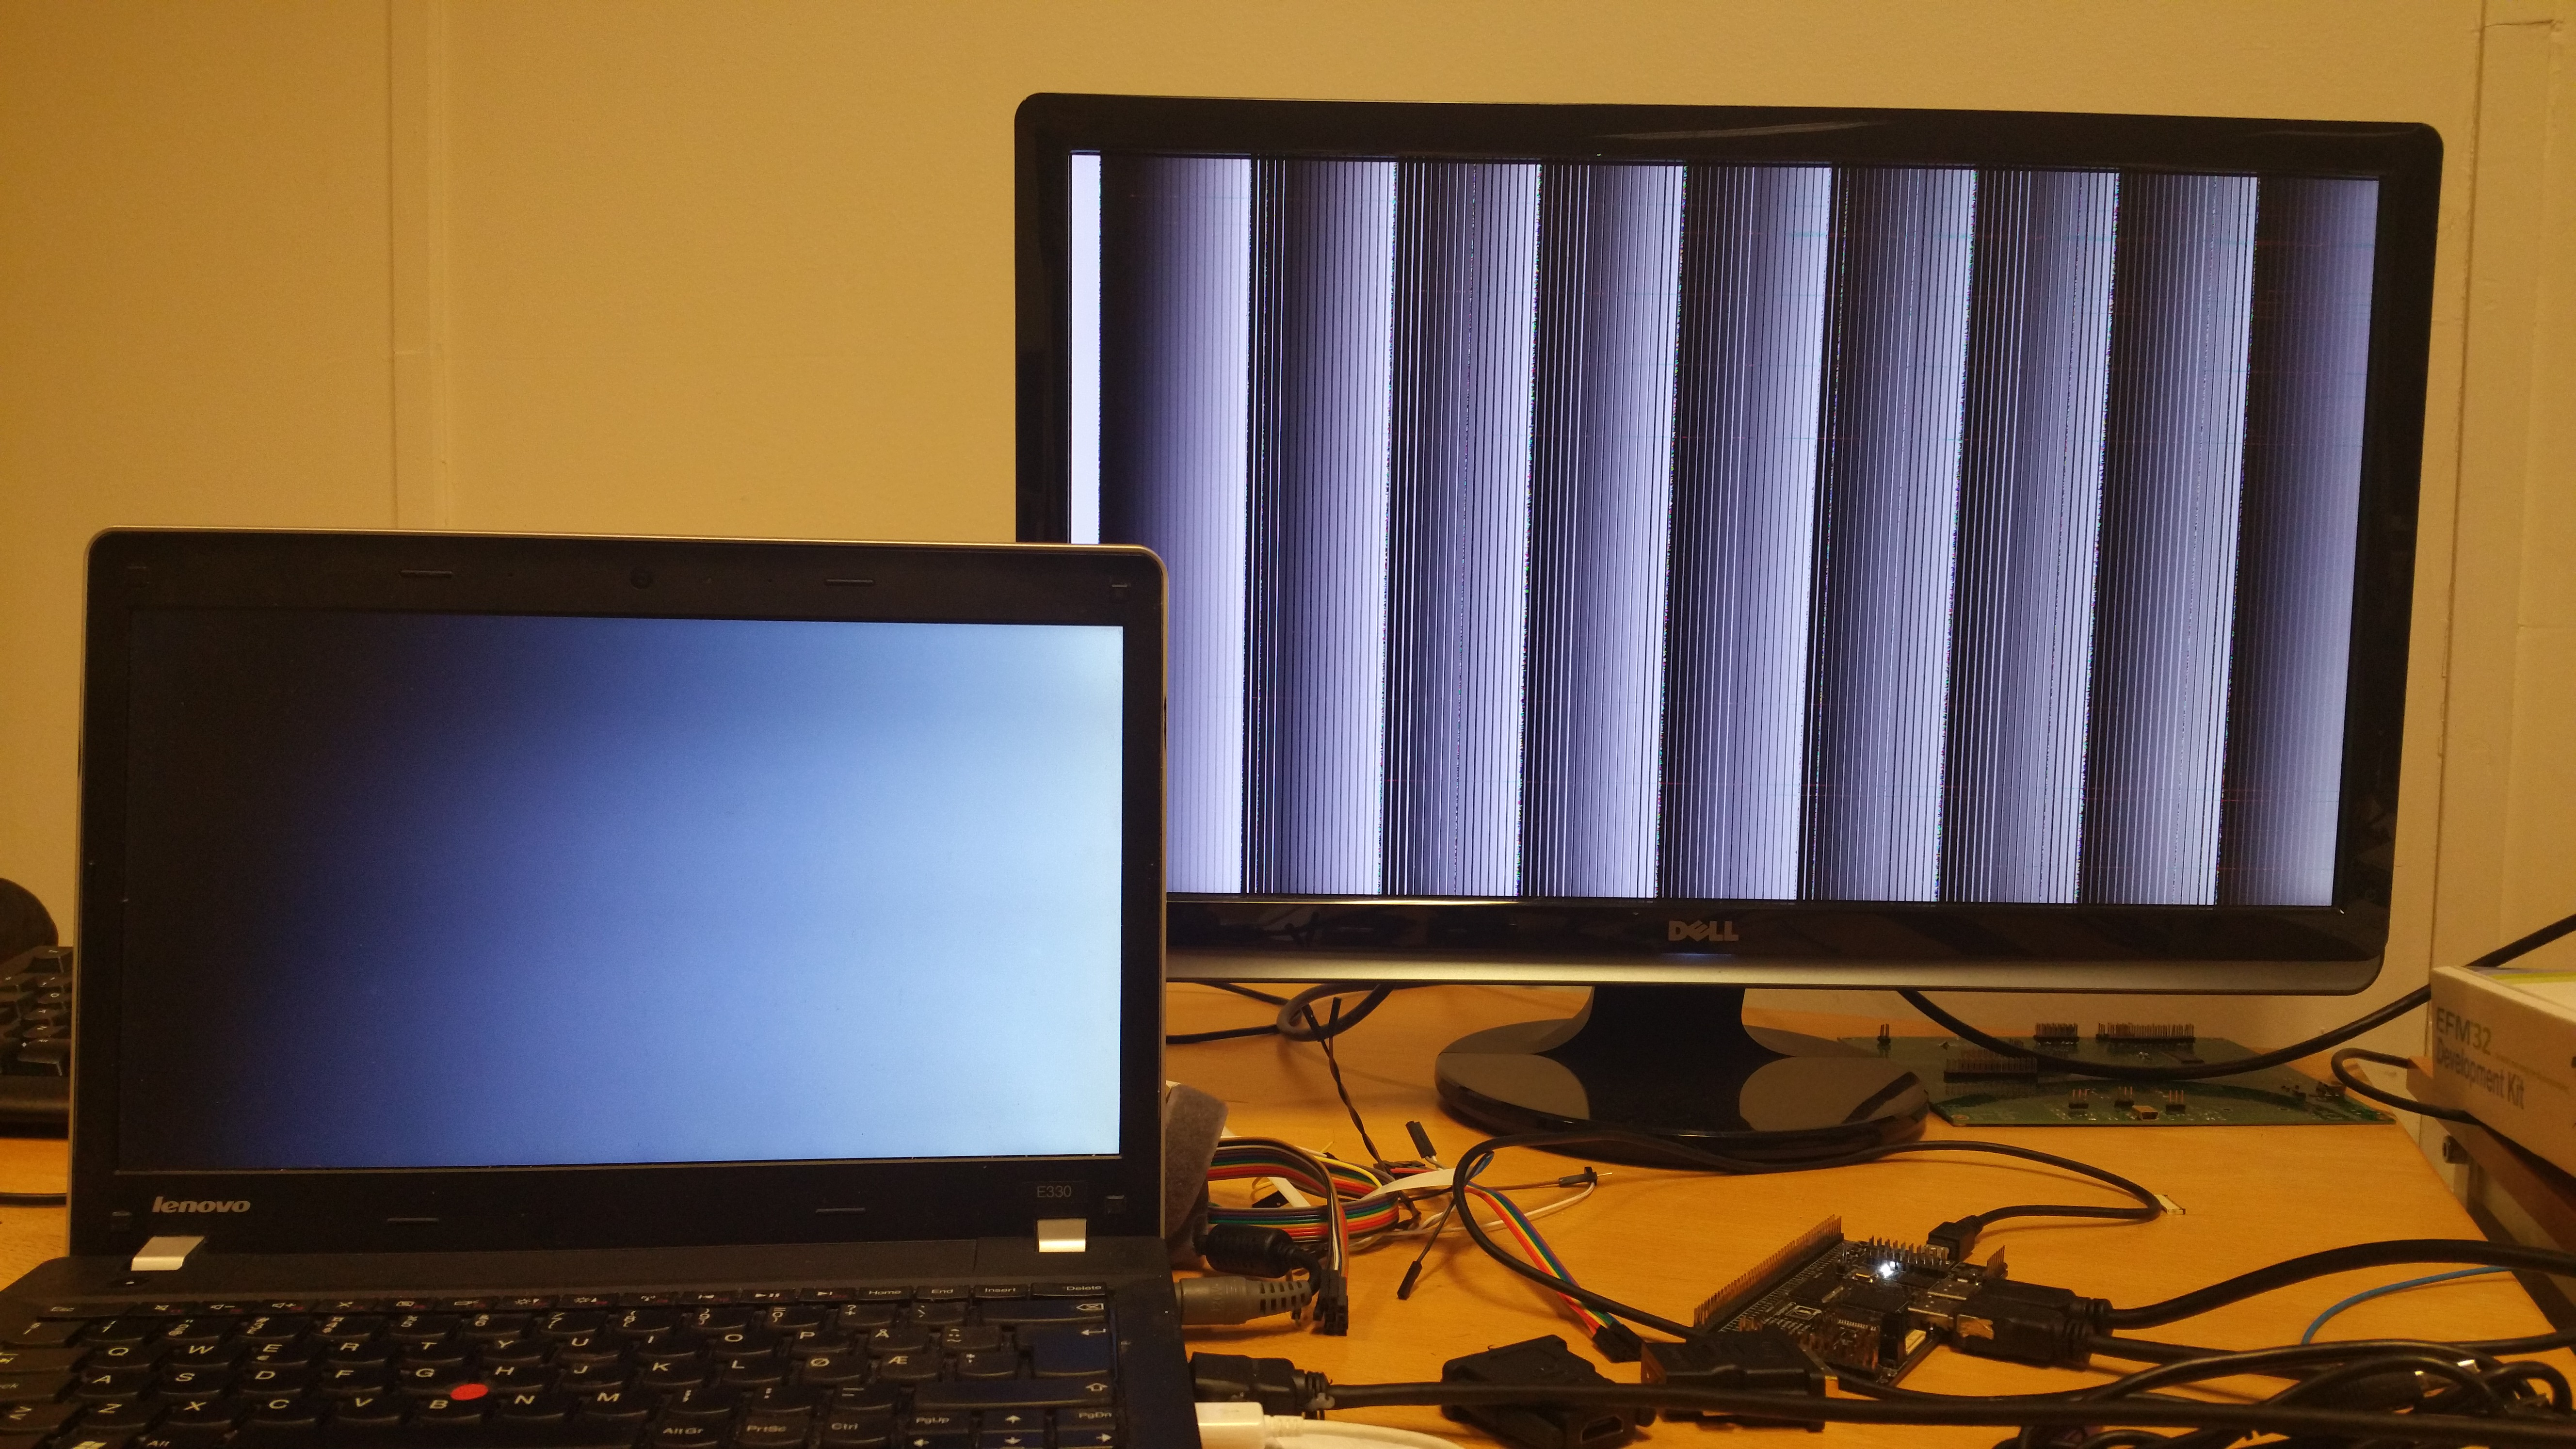
\includegraphics[width=14cm]{img/gradient_test}
    \caption[Gradient Output]{
        The laptop displays the input image, the display behind displays the output.
        The original gradient is turned into several shorter periods due to overflow when accumulating the final values.
        A 3x3 matrix of ones is used as kernel.
    }
    \label{fig:Overflow}

\end{figure}

\subsection{HDMI Channel Path}
After the first test of HDMI output from HDMI input, the HDMI input pins for R and B were swapped in the FPGA constraints to produce a picture with correct colour values.
The underlying problem were the HDMI output channels being swapped in the constraints. 
This led to the HDMI channel path for R and B through the FPGA to be remapped twice as shown in Figure \ref{fig:hdmiChannelPath}.
The image will have the correct colours at the output, but since VSYNC and HSYNC signals are only sent over channel B, information used to synchronize the image is lost.
By swapping the corresponding output channels instead of the input channel, a picture with correct colours as well as VSYNC and HSYNC signals appeared on the display.

\begin{figure}[h!]
    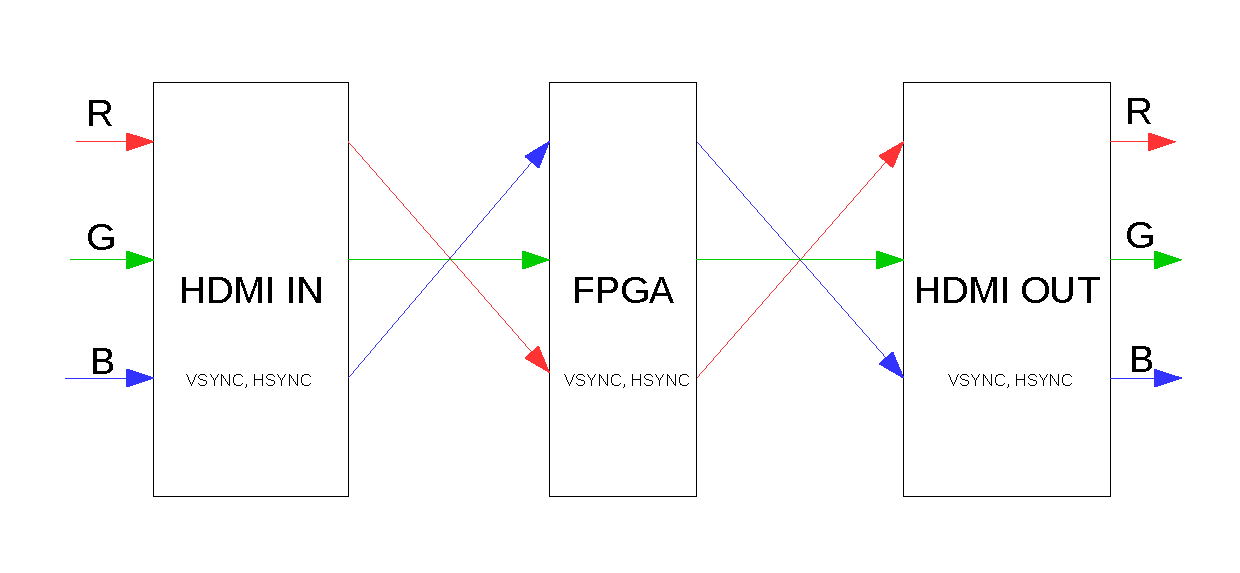
\includegraphics[width=\linewidth]{img/hdmi_channel_path.pdf}
    \caption[HDMI channels being swapped in the FPGA constraints]{
        HDMI channels being swapped in the FPGA constraints, VSYNC and HSYNC is lost
    }
    \label{fig:hdmiChannelPath}
\end{figure}

\subsection{Scalability}
What convolution kernel matrix sizes can be handled, what image resolutions and depths... TODO: Add more text.
As stated in Section \ref{sec:processor}, the processor has several parameters, some of which are hard coded into the final design.
These parameters can be adjusted, but many are limited by the available hardware.

According to the reports produced by Xilinx ISE during building of the FPGA bit file, the design for 3x3 convolution utilized around \unit[16]{\%} of the total number of available slices.
    This includes many slices with unused components.

    TODO:
    The same report states the processor can be clocked at a maximum frequency of \emph{<insert frequency>}. This was however tested in practice as the processor was expected to deliver data quickly enough at lower frequencies.

    \subsection{Video Throughput}
    The highest correctly working resolution was found to be 1366x768. This worked in real time with no perceivable delay. 1600x900 was also tried and found to be working, but resulted in an unexpected image with more artefacts. Finally, 1920x1200 was tried, but no sensible output was detected by the display.
